\clearpage
\section{Energy regressions for photons and electrons in the 2016 dataset}
\label{app:regression}

\newcommand{\Eraw}{\ensuremath{E_\text{raw}}\xspace}
\newcommand{\Etrue}{\ensuremath{E_\text{true}}\xspace}
\newcommand{\Ecorr}{\ensuremath{E_\text{corr}}\xspace}

The energy of reconstructed photons is measured by translating the detected amount of light in the scintillating lead-tungstate crystals into energy measurements, and summing the energy of crystals within a specified region called the \textit{supercluster}.
% 
This energy measurement yields what is called the \textit{raw energy} $\Eraw$; it is the baseline for further corrections, which are designed to approximate the \textit{true energy} $\Etrue$ as closely as possible.
% 
These corrections are required mostly to solve the lack of containment of the particle's energy deposit within CMS ECAL.
% 
For example, gaps in between the crystals and modules may cause some deposited energy not to be reconstructed, a problem referred to as limited \textit{local containment}.
% 
In addition, there is a non-negligible material budget in between the interaction point and ECAL, leading to photon conversions and brehmstrahlung for electrons.
% 
The radiated particles from these effects are typically bent along the $\phi$ direction due to the strong magnetic field, and may on occasion fail to be included in the determination of the supercluster~\cite{Chatrchyan:2013dga}.
% 
This problem is referred to as limited \textit{global containment}.
% 
The procedure of obtaining an estimate of $\Etrue$ from $\Eraw$ is called the \textit{energy regression}.


The regression is carried via a \textit{semiparametric boosted decision tree (BDT)}, which is a boosted decision tree that in its leafs carries a parametrization of the target.
% 
This type of multivariate analysis is called semiparametric as the product is parametric, but the decision tree itself is not.
% 
The parametric form chosen in the leafs is a so-called \textit{double-sided crystal ball function} (DCSB) function, with the following formulaic form~\cite{Aad:2015oqa}:
% 
\begin{linenomath*}
\begin{equation}
\text{DCSB}(x) = \left\{
    \begin{array}{ll}
    \exp{-\alpha_L^2/2}
        \left( 1-\frac{\abs{\alpha_L}}{n_L} \left(\abs{\alpha_L}+t\right) \right)^{-n_L}
        & \text{if} \quad t \leq -\alpha_L, \\
    % 
    \exp{-t^2/2} & \text{if} \quad -\alpha_L < t < \alpha_R, \\
    % 
    \exp{-\alpha_R^2/2}
        \left( 1-\frac{\abs{\alpha_R}}{n_R} \left(\abs{\alpha_R}+t\right) \right)^{-n_R}
        & \text{if} \quad t \geq \alpha_R, \\
    \end{array}
    \right.
\end{equation}
\end{linenomath*}
% 
where $t = \frac{x-\mu}{\sigma}$, and $\mu$, $\sigma$, $\alpha_{L/R}$ and $n_{L/R}$ are parameters of the DSCB; importantly, $\mu$ and $\sigma$ are the mean and standard deviation of the Gaussian core of the function.
% 
For the regression performed here, $\alpha_L$ has been fixed to 2, and $\alpha_R$ to 1; these constant values seem to work well throughout the energy regime, and fixing them allows the BDT to learn the more important parameters of the Gaussian core.
% 
The regression takes as input a number of variables from ECAL, such as the raw energy, the location of the supercluster in the detector, the width and height of the supercluster in terms of $\eta$ and $\phi$, and the ratio of the total energy measured in HCAL over the total energy measured in ECAL.
% 
The most important variables, however, pertain to the \textit{shower shape} of the electron or photon; notable examples include \textit{R9}, defined as the ratio of the summed energy of the $3\times3$-cluster around the electron/photon over the energy of the supercluster, and ratios of various crystal arrays over the summed energy of the $5\times5$-cluster around the electron/photon.
% 
In the case of electrons, a second set of variables is available from the tracker; these are mostly important for low-energy electrons.
% 
The regression is performed separately for the barrel and endcap regions, and as such the input variables also differ slightly; for example, in the endcap regions the preshower energy measurement is included as an input, and rather than $\eta$ and $\phi$, the location of the superclusters are given in planar coordinates.


For low-energy electrons, the most prominent variables for the energy correction are those from the tracker.
% 
While an obvious fact from physics concerns, in a BDT these type of trivialities must be learned through the analysis of large amounts of data.
% 
In order to speed up the training, increase chances of convergence and to improve the final result, it is typically preferable to design the training with these given facts in mind.
% 
The energy regression for electrons is determined by first training a BDT using only ECAL variables.
%
As a target function, which is to be brought as closely to 1 as possible with minimal standard deviation per leaf, it uses
% 
\begin{linenomath*}
\begin{equation}
\text{target}_1 = \frac{\Etrue}{\Eraw}
\,.
\end{equation}
\end{linenomath*}
% 
The corrected energy $\Ecorr$ that is yielded by this BDT is already a good estimate of $\Etrue$, and for energies $>100\GeV$ it is basically the final estimate.
% 
Subsequently, a second BDT is trained, this time including the tracker variables, with the target defined as
% 
\begin{linenomath*}
\begin{equation}
\text{target}_2 = 
% 
\frac{\Etrue}{E_\text{estimate}} =
% 
\frac{\Etrue}{ w_\text{ECAL} \Ecorr + w_\text{tracker} \abs{p} }
\,,
\end{equation}
\end{linenomath*}
% 
where $\abs{p}$ is the absolute momentum determined from the tracker, and the weights are defined as
% 
\begin{linenomath*}
\begin{equation}
w_\text{ECAL} = \left( \frac{\sigma^2_{\abs{p}}}{\sigma^2_{\abs{p}} + \sigma^2_{\Ecorr}} \right)
\;,\quad
w_\text{tracker} = \left( \frac{\sigma^2_{\Ecorr}}{\sigma^2_{\abs{p}} + \sigma^2_{\Ecorr}} \right)
\,.
\end{equation}
\end{linenomath*}
% 
The denominator is essentially a weighted sum of the energy estimations from the tracker and from ECAL, where the weights are determined by the respective uncertainties.
% 
With this two-tiered approach, the regression has only to learn in the second stage to trust the tracker energy estimate more for low-energy electrons, and the ECAL estimate for high-energy electrons, greatly reducing the required training time and improving the chances for convergence.
% 
Histograms of the weights for increasing electron $\pt$ are shown in Fig.~\ref{fig:regressionweights}; for very low $\pt$, the tracker weight is typically larger, whereas for a larger $\pt$ the weight assigned to the corrected ECAL energy measurement is larger.


With respect to previous versions of this regression (meant for data collected by the CMS detector before 2016), the results described here include variables pertaining to \textit{crystal saturation}, the effect that occurs when the deposited energy exceeds the maximum allowed value of the analog-to-digital converter.
% 
This effect occurs for energy deposits greater than approximately $2000\GeV$, and severely deteriorates the energy scale and resolution.



\begin{figure}[hbtp]
  \begin{center}
    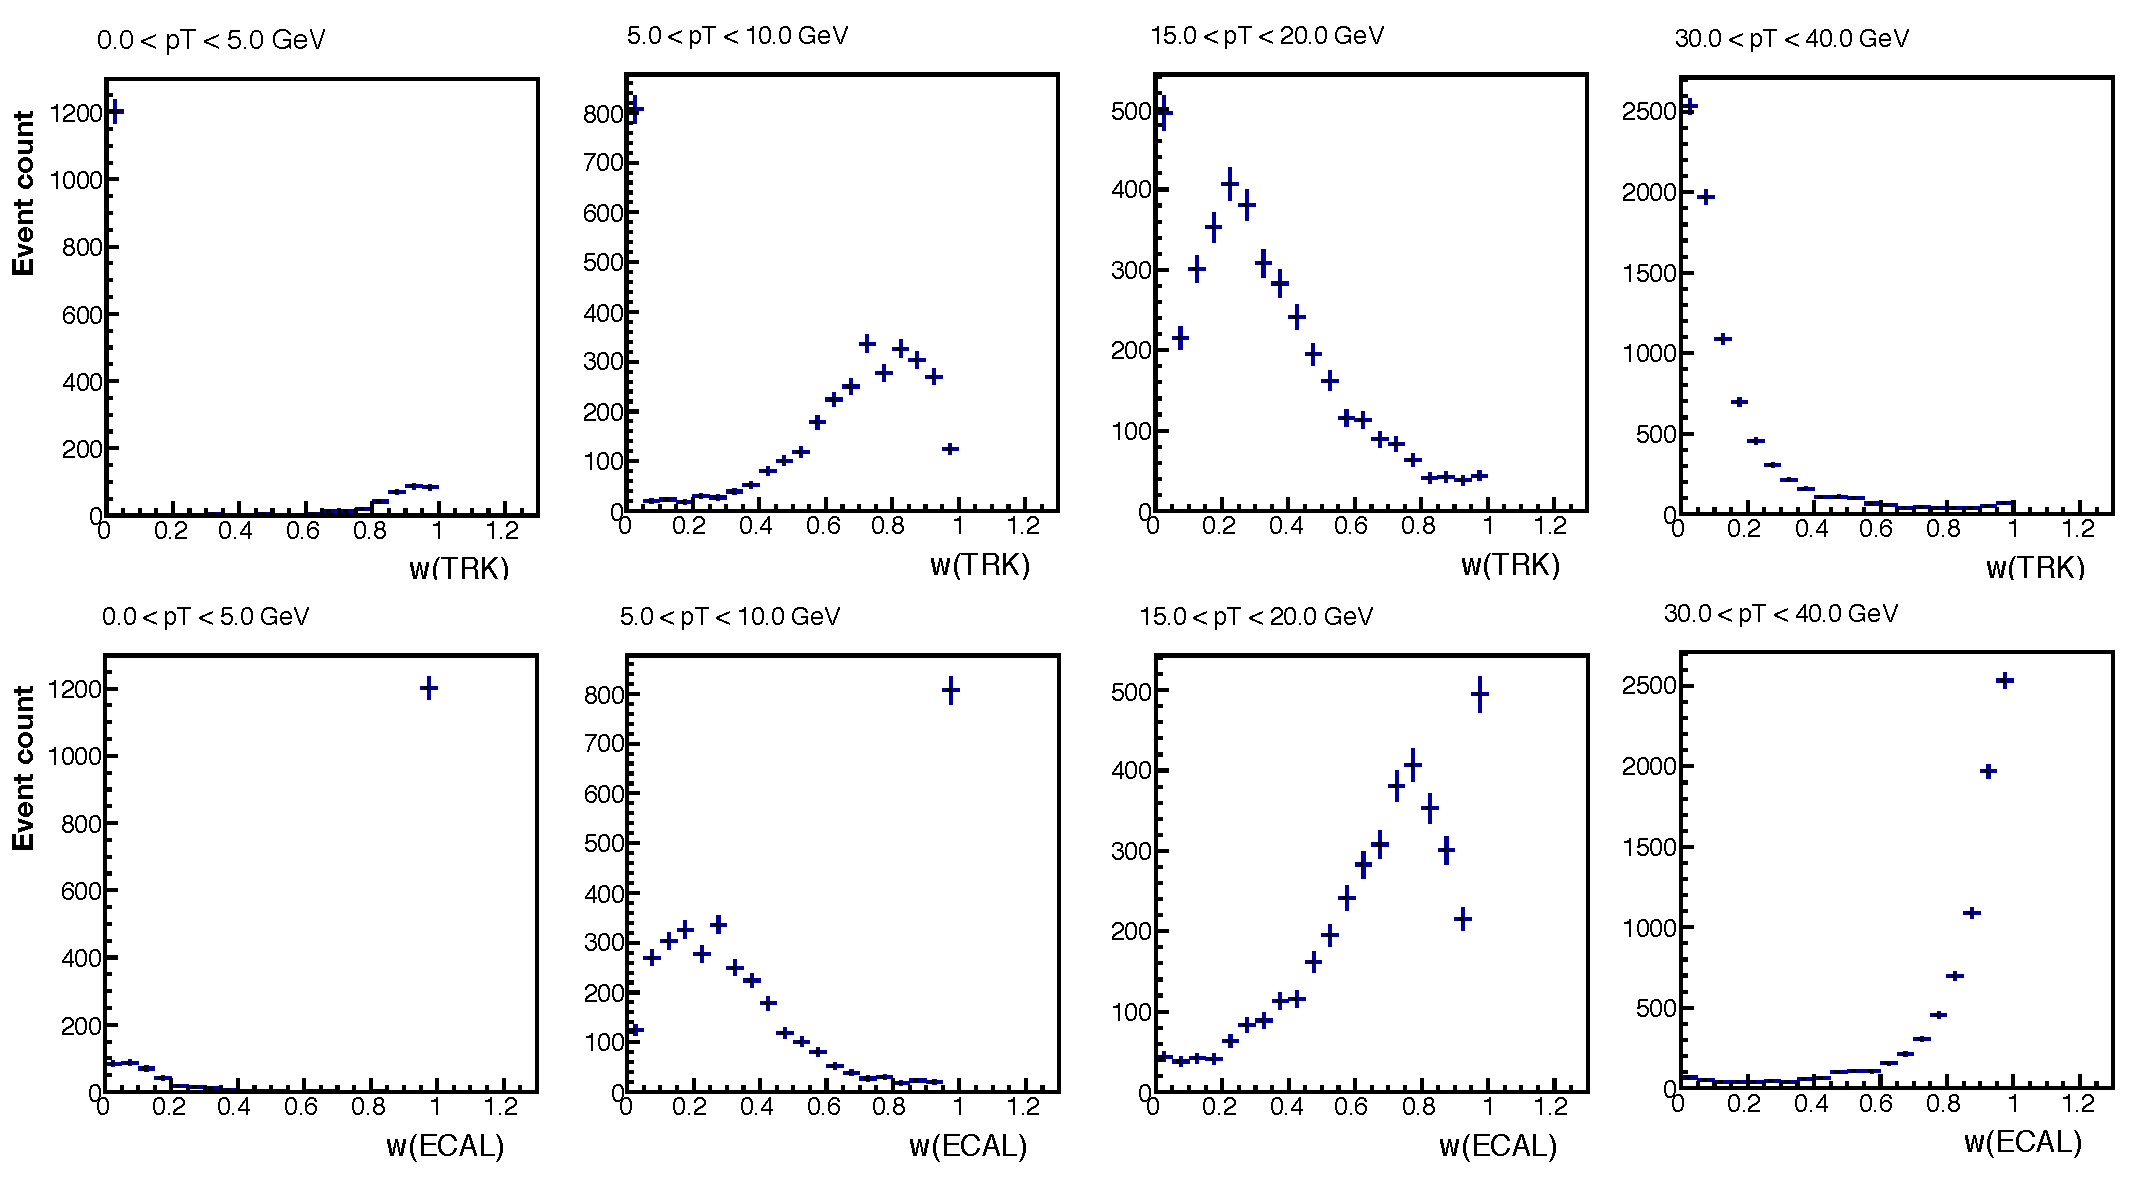
\includegraphics[width=0.99\linewidth]{img/regression/weightplot.pdf}
    \caption{
        Weights based on uncertainties in energy resolution for the tracker energy measurement (top row) and the ECAL energy measurement (bottom row), for increasing electron $\pt$.
        %
        For larger electron $\pt$, the weight assigned to the corrected ECAL energy measurement from the first BDT is larger, whereas for small electron $\pt$ the weight assigned to the energy estimate from the tracker is larger.
        % 
        For a particular subset of events, the tracker energy resolution is, by chance, very poor; this leads to a nearly full weight placed on the ECAL energy measurement in these cases, visible as a peak at 1.0 in the $w_\text{ECAL}$ histograms.
        }
    \label{fig:regressionweights}
  \end{center}
\end{figure}

